\chapter{Metodologia}
\label{ch:metodologia}

Tavoiteltu lopputulos on malli, joka palauttaa stereokuvasta syvyysdatan ilman liikkuvia kohteita.
Manuaalisesti tämän voisi toteuttaa laskemalla kuvista dispariteetti ja poistamalla tästä dispariteetti kuvasta halutut kohteet.
Jos lähtökohtana on kuvapari, on manuaalinenkin arviointi hyvin likimääräistä. Kuitenkin voidaan ajatella, että perusperiaatteeltaan asioiden takana oleva syvyys jatkuu samanlaisena kuin asian ympärillä.
Vaikka tämä ei aina päde, pyritään mallilla testaamaan, onko kappaleen täyttö sitä ympäröivillä syvyyksillä riittävä tekniikka.

\section{Stereoanalyysi}

Syvyysdatan ja dispariteetin analysointi tehdään ilman neuroverkkoja.
Tässä tapauksessa Hirschmullerin SGM-algoritmillä \cite{hirschmuller2005babel}.
Käytettävä variaatio tästä algoritmista on OpenCV:ssä toteutettu StereoSGBM \cite{opencvsgbm}.
Seuraava esimerkki Kuva \ref{fig:disparity1} on luotu funktion parametreillä: numDisparities=128, blockSize=20, mode=cv2.StereoSGBM\_MODE\_HH,
sekä lisäämällä stereokuviin gaussinen sumennos laskennan helpottamiseksi \cite{AnShiyong2021Asvs}.

\begin{figure}[h]
\centering
\pdftooltip{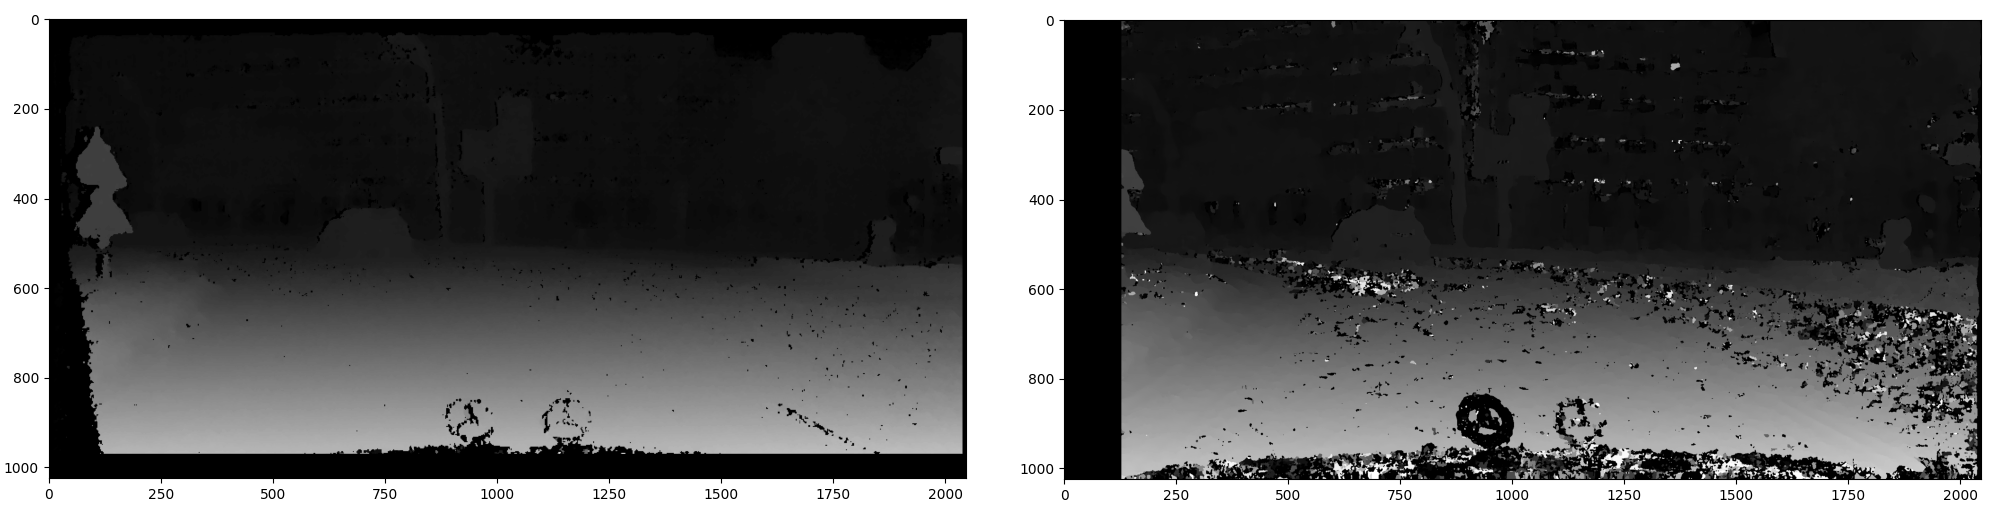
\includegraphics[width=\textwidth]{figures/disparity_1.png}}{disparity example}
\caption[Tämä on lyhyt kuvateksti.]{Vasemmalla tarjottu totuus. Oikealla OpenCV:n tulos stereokuvasta.}
\label{fig:disparity1}
\end{figure}
    
Syvyysdatan kerääminen stereokuvista on mahdollista OpenCV2-kirjaston avulla.
Sumennus lisättiin, jotta mahdolliset kameran aiheuttamat häiriöt saadaan minimoitua.
Käytetyt parametrit tarkoittavat sitä, että mahdollisia "disparity" tasoja on 128 ja alue jolta samankaltaisuutta verrataan on 20 pikselin kokoinen.
Funktiota ajettiin HH-modessa, joka tarkoittaa, että se suoritetaan algoritmin alkuperäisellä suoritustavalla, 
eikä kevennetyllä, jota käytetään muistin säästämiseksi.

Tuloksestamme huomaamme häiriötä jota totuudessa ei ole.
Tämä johtuu todennäköisesti kuvissa olevista kohdista, joita Hirschmullerin-algoritmi ei pysty tunnistamaan toisesta kuvasta.
Tämä voi tapahtua esimerkiksi asfaltin pinnassa tai varjoisilla alueilla, jossa kuva näyttää samalta suurella alueella.

Tässä tilanteessa voisimme myös kouluttaa verkon, jonka avulla saisimme hankittua syvyysdataa.
Toisaalta syvyysdata ei ole yleisesti saatavilla olevaa koulutusdataa,
joten ei voida olettaa, että se olisi saatavilla tulevissa toteutuksissa. 

\section{Semanttinen Segmentointi}

Aineistossa on jo olemassa totuus segmentaatiodatasta.
Käytämme tätä valmista dataa, mutta koulutamme silti sitä varten myös uuden verkon.
Koulutettu verkko on hyvin yksinkertainen ja käyttää valmiita PyTorch-komponentteja.
Data on koulutettu\ fcn\_resnet50 avulla \cite{pytorchfcnresnet50}, ilman esikoulutettuja painoja. Optimointiin on käytetty Adam-algoritmia ja häviöfunktioksi on valittu CrossEntropyLoss-funktio.
Datasetin mallia on yksinkertaistettu tarpeen mukaan: kaikki liikkuvat kohteet, kuten autot ja ihmiset, on yhdistetty yhdeksi luokaksi ja kaikki muu toiseksi luokaksi.
Näin saadaan yksinkertaisempi malli, jonka avulla voidaan kuvasta tunnistaa kaikki liikkuvat kohteet Kuva \ref{fig:segmentation1}.

\begin{figure}[h]
\centering
\pdftooltip{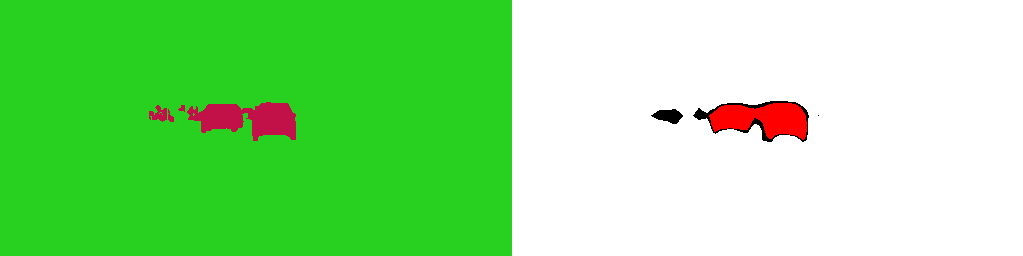
\includegraphics[width=\textwidth]{figures/segmentation1.png}}{segmentation example}
\caption[Tämä on lyhyt kuvateksti.]{Vasemmalla tarjottu totuus. Oikealla mallin tuottama.}
\label{fig:segmentation1}
\end{figure}


Tällä tavalla tehty malli antaa meille riittäviä tuloksia alkuperäiseen totuuteen verrattuna.
Sen kouluttaminen on myös melko yksinkertaista.
Tätä mallia ei kuitenkaan tarvita lopullisen mallin luomiseen niissä mahdollisissa käyttökohteissa, joissa dataa ei ole saatavilla.
Voi kuitenkin olla helpompaa segmentoinnin sijaan arvioida suoraan asioiden alla oleva syvyys.
Mikäli data tuotetaan esimerkiksi useilla kuvilla samoista kohdista, joissa kohteet liikkuvat,
on segmentaatiomallista enemmän hyötyä.
Sitä voisi tämän kaltaisissa tapauksissa käyttää pelkästään taustasyvyysarvioinnin tuottamiseen ilman syvyyksien arvaamista.

\section{Datan muodostus}

Tämän työn tavoite on jalostaa data muotoon, jossa kaikki liikkuvat kohteet on hävitetty syvyysdatasta.
Koska käytetty data on kaupunkidataa, tämä tarkoittaa autojen sekä ihmisten poistamista kuvista.
Koska käytettävissämme on kuvien segmentaatiodata, voidaan niiden alue poistamalla dispariteetista saavuttaa tila, jossa niitä ei oteta huomioon.

Kun liikkuvien objektien alue on poistettu, pitää niiden alla oleva alue generoida jotenkin,
koska alueiden alla voi olla miltei mitä tahansa,
eikä meillä ole selkeää keinoa sitä tietää. 
Alueen alle voi jäädä taloja joissa on erikoisia kulmia, puita, pensaita, postilaatikoita, tolppia ja mitä tahansa muuta. 
Näistä syistä ei voida olettaa, että kyseinen malli olisi erityisen tarkka, 
mutta alueen karkeaan arviointiin tuotetun datan pitäisi olla riittävä.
On tärkeä muistaa, että huonosti toteutettu datasetti tuottaa myös huonoja tuloksia tuottavan mallin.

Tässä vaiheessa mallin käsittelyä yritettiin vertikaalisella ja horisontaalisella pyyhkäisyllä, sekä niiden yhteistuloksella.
Näin ollen jokainen yhtenäinen alue etsittiin ja niiden syvyysarvot otettiin niiden reunoilta
ja pyyhkäistiin läpi täsmäämään vastakkaisen reunan arvoon.
Tästä seuraa, että jos kohteen takana on esimerkiksi puu, vertikaalinen pyyhkäisy osaisi ottaa sen huomioon.
Jos kohteen takana sen sijaan on aita, horisontaalinen pyyhkäisy osaisi ottaa sen huomioon.
Ja yhdistetyssä tavassa nämä arvot on summattu, joten sen pitäisi olla keskiarvoltaan hyvä. 

\begin{figure}[h]
    \centering
    \pdftooltip{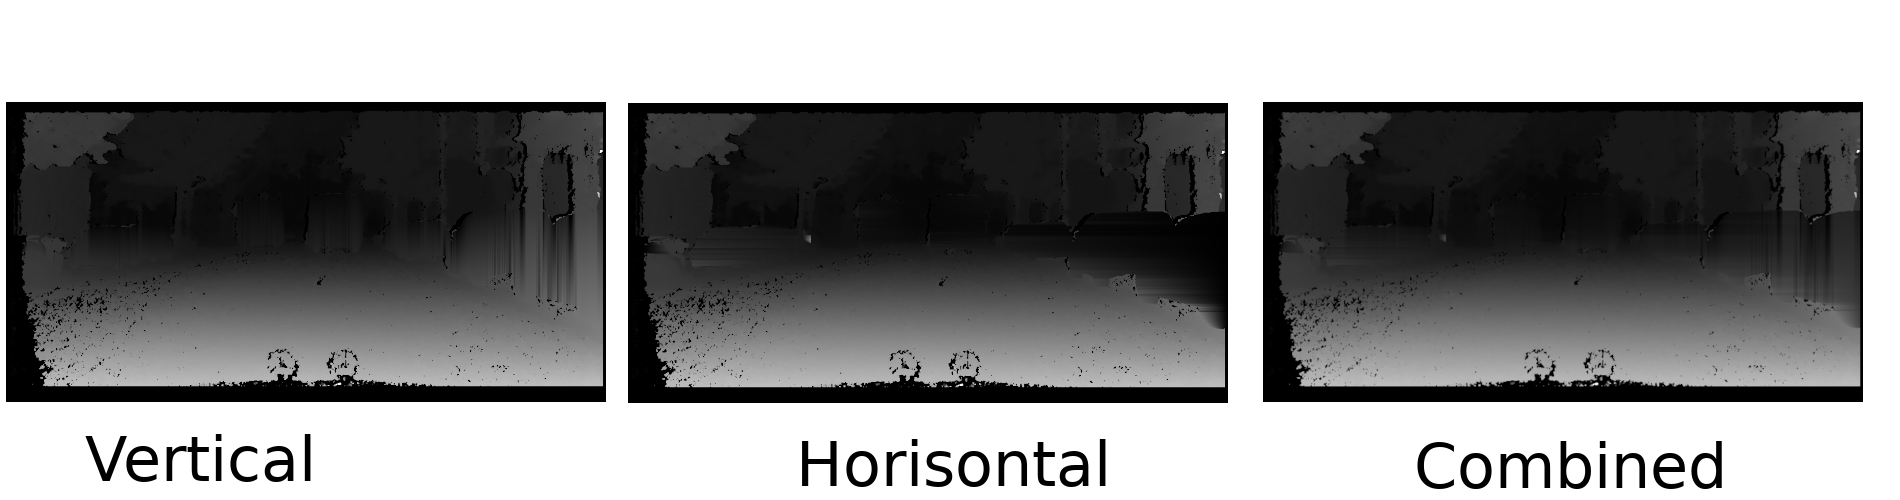
\includegraphics[width=\textwidth]{figures/swipe.png}}{Swipe}
    \caption{Eri tyypin pyyhkäisyt syvyyden arviointiin}
    \label{fig:swipe}
\end{figure}

Tässä kuvassa Kuva \ref{fig:swipe}, on esitelty tavat vertikaali, horisontaali sekä niiden yhdistetty arvo. 
Kuvasta huomataan, että mikään tavoista ei ole täydellinen,
ja jotta datasta saadaan edes jollain tavalla käytettävää, tulee se ensin tarkistaa. 

\begin{figure}[h]
    \centering
    \pdftooltip{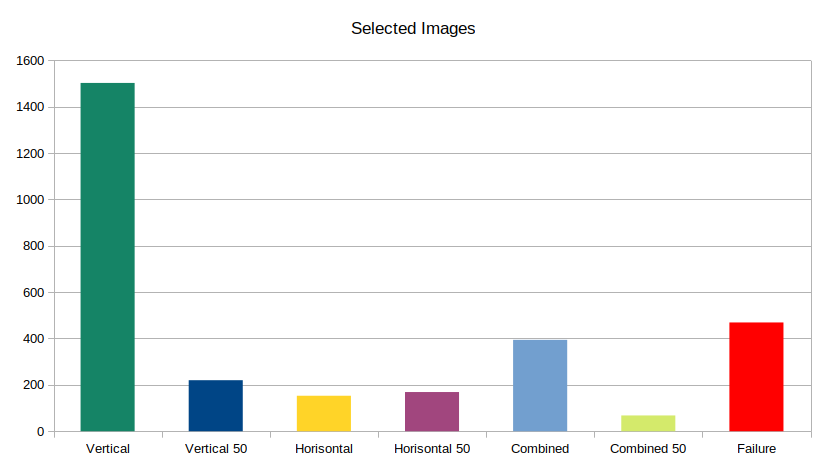
\includegraphics[width=\textwidth]{figures/selectedimages.png}}{Selected}
    \caption{Valitut kuvat}
    \label{fig:selected}
\end{figure}


Kuvien manuaalisessa valinnassa vertailtiin yllä mainittujen kuvien lisäksi pyyhkäisyjä,
jotka ylittävät tunnistetun reunan 50:llä pikselillä.
Datan läpikäynnin jälkeen valituksi tuli seuraavanlaisia kuvia Kuva \ref{fig:selected}.


Tästä huomaamme, että vertikaalisen valinnan olevan yleisin.
Mikäli horisontaalista dataa tarvittiin, se yleensä kannatti yhdistää vertikaalidataan.
Tämä johtuu todennäköisesti datan luonteesta. Suuri osa kohteista on melko lähellä kameraa ja reunassa, 
mikä johtaa tilanteeseen, jossa analysoitavan alueen oikealla tai vasemmalla puolella ei ole tarpeeksi syvyyden generoimiseen tarvittavaa dataa.
Vertikaalipyyhkäistyjen kuvien data on myös todennäköisemmin oikein, koska suurin osa datasta on eteenpäin jatkuvalta tieltä.
Näin ollen ylempänä kuvassa oleva kohde on usein kauempana.
Tästä johtuen vertikaalinen pyyhkäisy on todennäköisemmin oikein kuin vasemmalta oikealle tuleva, joka näyttäisi tuovan tulokseen enemmän satunnaisuutta.
Koska kuvat on käsin silmämääräisesti valittuja, luonnollisimman näköiset kuvat tulevat todennäköisemmin valituiksi.
Yhden kuvan valitsemiseen ei kuitenkaan ole käytetty paljoa aikaa, vaan valinta oli hyvin ”fiilispohjaista”.

Ongelmia aiheutti yleisemmin segmentoitujen alueiden vieressä olevat epäselvyydet sekä alueet, jotka olivat niin reunassa, ettei niiden vierestä käytettävän syvyyden saanti ollut mahdollista.

Jatkokehityksessä edellä mainittuja ongelmia voisi yrittää parantaa muutamilla tavoilla. 
Tunnistettuja alueita laajentamalla voisimme onnistua piilottamaan joitain tunnistettujen alueiden reunoilla esiintyviä syvyysdatan häiriöitä.
Koska emme ole kiinnostuneita tunnistamaan asioita vaan piilottamaan ne, ei kovin suuri tarkkuus ole tarpeellista.
Jälkianalysoinnin kannalta myös liian suuri alue on huomattavasti pienempi harmi kuin liian pieni alue.

Lisäksi tulosta voisi parantaa siistimällä dispariteettidatasta kohinaa suodattamalla.
Tämä todennäköisesti poistaisi myös jotain tärkeää dataa,
mutta jälleen kerran tavoiteltu tarkkuus ei ole niin suuri, että tästä pitäisi koitua suuresti haittaa.

Koulutusdatan kuville voitaisiin myös luoda syvyyttä arvioiva kehys.
Tämä varmistaisi sen, että syvyys on aina saatavilla, 
ja tällaisen kehyksen generointi pitäisi olla mahdollista datan samankaltaisuudesta johtuen.

Yksi yleisesti ongelmia tuottava tunnistettu kohde ovat ihmiset.
Ihmiset ovat monimutkaisempia muotoja kuin autot.
Näin ollen myös mallissa ihmisen erottelu on tarkempaa.
Kuitenkin joissain kuvissa,
jos ihminen peitetään pienimmän ja suurimman koordinaatin peittävällä kuutiolla,
menetetään paljon dataa, jota ihmisen ympäriltä on havaittavissa.
Tätä varten voisi olla hyödyllistä kirjoittaa algoritmi, joka arvioisi muutoksen alueella olevia suurimpia eroja ja suodattaisi suurimmat muutokset pois.
Näin menetettäisiin osa datasta,
mutta todennäköisesti myös suurimmat virheet saataisiin hävitettyä. 

Tällä tavalla tuotettu malli vaatii paljon manuaalista työtä ja hyväksyntää.
Kun uusia malleja tehdään, niiden luomiseen ei ole oikoteitä.
Mitä enemmän tätä työtä tehdään,
sitä helpommaksi se olemassa olevan mallin avulla tulee.
Manuaalisesta työstä ei kuitenkaan koskaan pääse datan validoinnissa pois,
mikäli käytössä ei ole parempaa lähtödataa.
Jos datasetti muodostettaisiin ottamalla samasta kohdasta useita kuvia,
kunnes kaikki liikkuvat kohteet olisivat poistuneet,
voitaisiin sen ja segmentaatiomallin avulla luoda huomattavasti parempaa koulutusdataa. 

\section{Ensimmäinen malli}

Datasta koulutettiin malli samalla PyTorchin tarjoamalla "fcn\_resnet50" \cite{pytorchfcnresnet50} neuroverkolla kuin segmentaatiovaiheessa.
Ulostulon muoto jaettiin 128 luokkaan, jotka vastaavat eri syvyyttä.
Sisääntulona annettiin kaksi harmaata kuvaa 3-ulotteisen matriisin eri kerroksissa.
Näin voitiin käyttää valmista segmentaatiomallia värikuvasisääntulolla kahden stereo-mustavalkokuvan analysointiin ja tuottaa sillä syvyyskartta.

\begin{figure}[h]
\centering
\pdftooltip{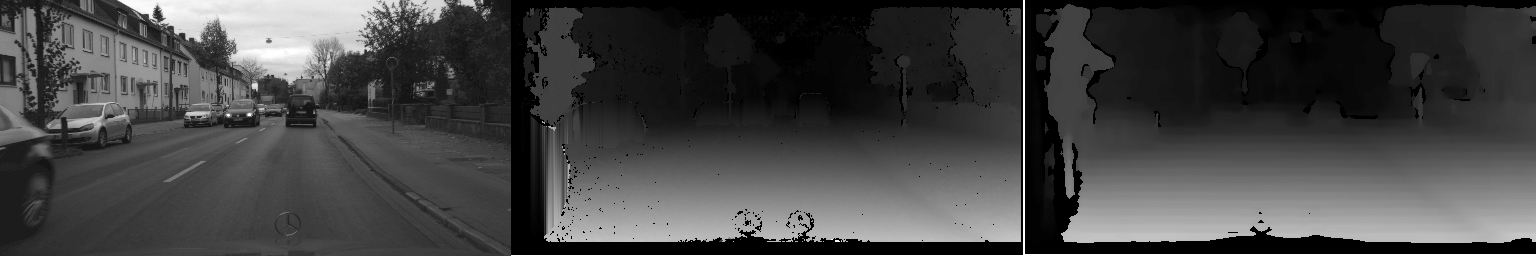
\includegraphics[width=\textwidth]{figures/model.png}}{Model}
\caption{Kuvassa vasemmalta oikealle; alkuperäinen kuva, rakennettu totuus, koulutetun mallin lopputulos.}
\label{fig:model}
\end{figure}

Kuvasta Kuva \ref{fig:model} nähdään, että koulutus itsessään pystyy tuottamaan hyvin samankaltaisia kuvia kuin laskettu malli. Koulutettu malli kuitenkin oletetusti perii koulutusdatan heikkoudet. Koska käytetty automatisoitu tapa ei tuota täydellistä dataa, ei myöskään koulutettu malli ole täydellinen. 

\section{Datan jatkojalostus}

Jotta mallista saataisiin parempi, täytyy koulutusdataa pyrkiä jalostamaan tehokkaammin. 
Aikaisemmat prosessointitavat olivat melko yleisiä ja käytettäviä millä tahansa datalla.
Paremman lopputuloksen saamiseksi olisi tarpeellista käyttää erikoistuneempia datankäsittelytapoja.
Käytetty koulutusdata oli kaupunkidataa ja tästä johtuen hyvin homogeenistä.
Voimme käyttää tätä hyväksemme yrittäessämme arvioida kohteiden takana olevaa syvyyttä.

\begin{figure}[h]
\centering
\pdftooltip{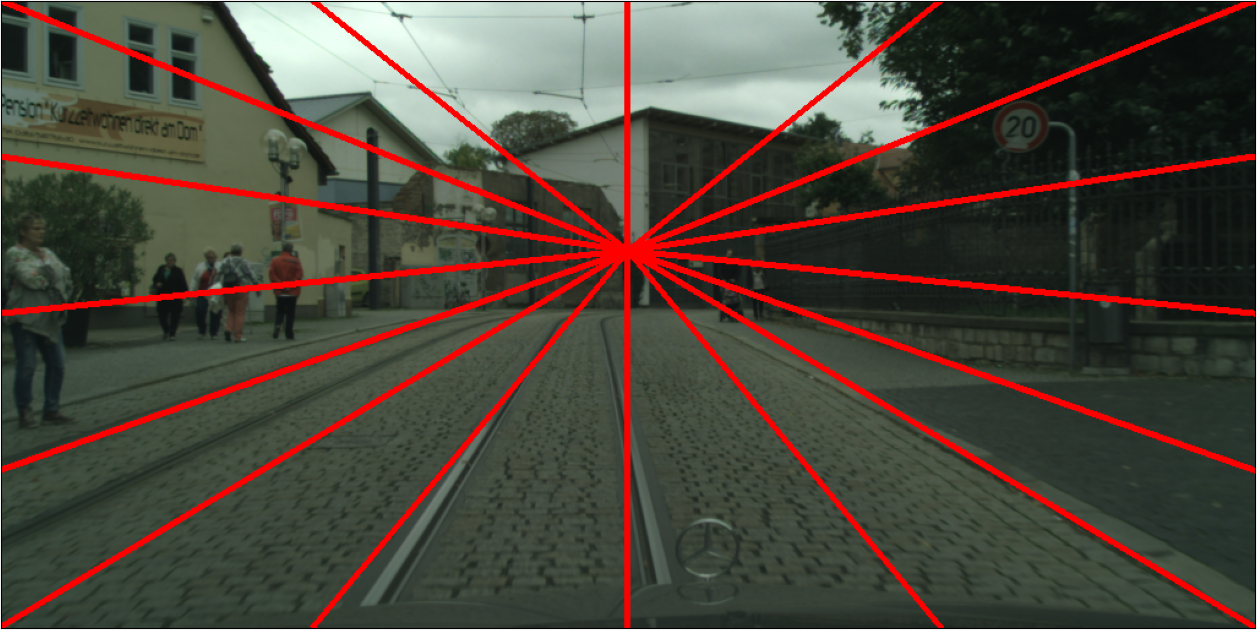
\includegraphics[width=\textwidth]{figures/focal_image.png}}{Model}
\caption{Kuvassa Esimerkki "polttopisteestä"}
\label{fig:polttopiste}
\end{figure}


Kaupunkiympäristössä kuva on usein otettu samankaltaisesta asetelmasta tiellä ajavasta autosta. 
Tästä johtuen voimme arvioida syvyyden muutoksen tapahtuvan hyvin samankaltaisesti eri kuvausajankohtina.
Tämän arvion voimme tehdä arvioimalla "polttpisteen" jossa todennäköisesti on kuvan suurin syvyys Kuva \ref{fig:model},
poislukien taivas, eli ainakin kuvan merkitsevän alaosan osalta.
Vaikka esimerkkikuvassammekaan syvyys ei asetu täysin arvioituun kohtaan,
on se silti tarpeeksi lähellä jotta sitä voitaisiin käyttää. 
Kun yhdistämme tähän geneerisissä tavoissa käyttämämme pyyhkäisytekniikan, jonka suoritamme polttopisteen suuntaan, 
saamme aikaan syvyyden muutoksen joka on luonnollisemman oloinen todelliseen syvyysdataan nähden.

Edellisen lisäksi voimme lisätä arvion syvyydestä kuvan eri alueilla. 
Tällöin on mahdollista syvyyden arviointi tilanteissa joissa korvattava kohde alkaa jo kuvan reunalta.

\begin{figure}[h]
\centering
\pdftooltip{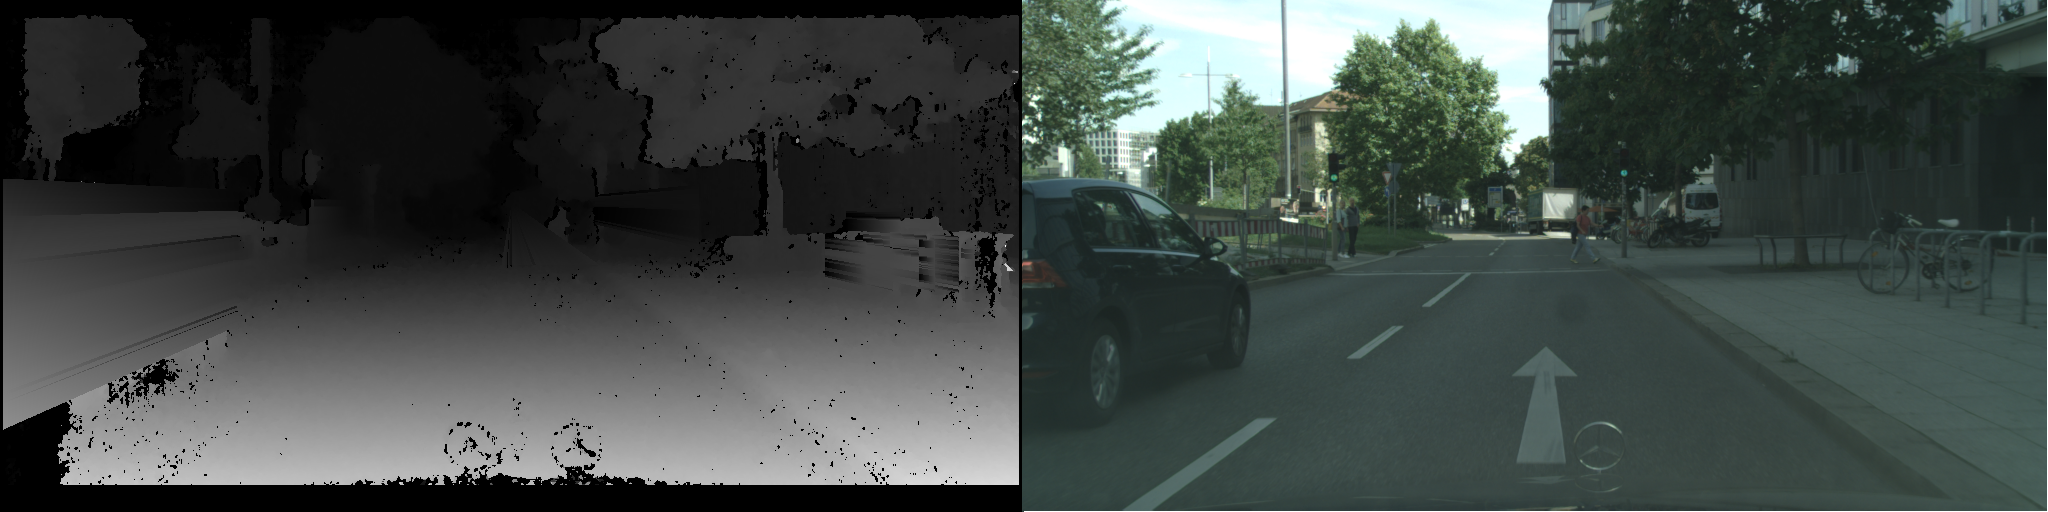
\includegraphics[width=\textwidth]{figures/focal_depth.png}}{Model}
\caption{Esimerkki syvyyden arvioinnista polttopistettä kohti}
\label{fig:polttopiste_2}
\end{figure}

Kuvassa \ref{fig:model} näemme vasemmassa reunassa olevan auton sijoittuvan aivan kuvan reunaan, 
emmekä näin ollen voi kuvasta tarkistaa alkavaa syvyyttä ennen autoa.
Tässä voimme käyttää likimääräisiä arvioita syvyyksistä kuvan eri alueille. Vaikka saatu lopputulos ei ole täydellinen,
on se silti toimiva lähtökohta syvyyden korvaamiselle.

Koska kyseessä on pelkästään käyttämäämme dataa varten valittu tekniikka, ei se tuota hyviä tuloksia kuin ainoastaan sen kanssa yhteensopivaan dataan.
Vaikka suuri osa datasta onkin keskenään samankaltaista, ei kuitenkaan kaikkien kuvien prosessointi ole järkevää sen avulla.
Manuaalisen läpikäynnin jälkeen huomaamme, että kuitenkin vain noin neljäsosa kuvista on tuottanut parhaan prosessointi lopputuloksen "Focal" eli polttopistetekniikan avulla. 

\begin{figure}[h]
\centering
\pdftooltip{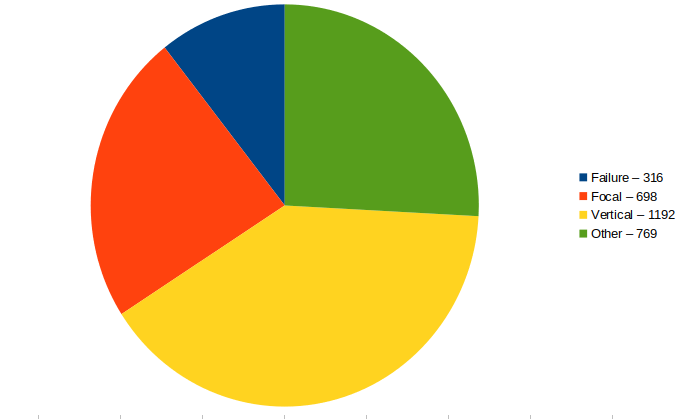
\includegraphics[width=\textwidth]{figures/NewChart.png}}{Selected2}
\caption{Uudet Valitut kuvat}
\label{fig:selected2}
\end{figure}

Uusi tapa on kuitenkin ratkaissut osan kuvista joiden reuna alueet ovat olleet täynnä autoja, siirtäen ne epäonnistuneiden kuvien joukosta käytettäviin kuviin.

\section{Lopullinen malli}

Lopullinen tuotettu malli on tehty samalla tavalla kuin ensimmäinenkin, 
sen kouluttamiseen on vain käytetty hieman erilaista dataa.
Mallin toiminnan paremmuuden tieteellinen analysointi ei kuitenkaan anna realistisia lopputuloksia, 
koska alkuperäinen data sisältää niin paljon häiriötä ja epäpuhtauksia, että sen arvioinnin tarkkuus on hyvin hankalaa.

\begin{figure}[h]
\centering
\pdftooltip{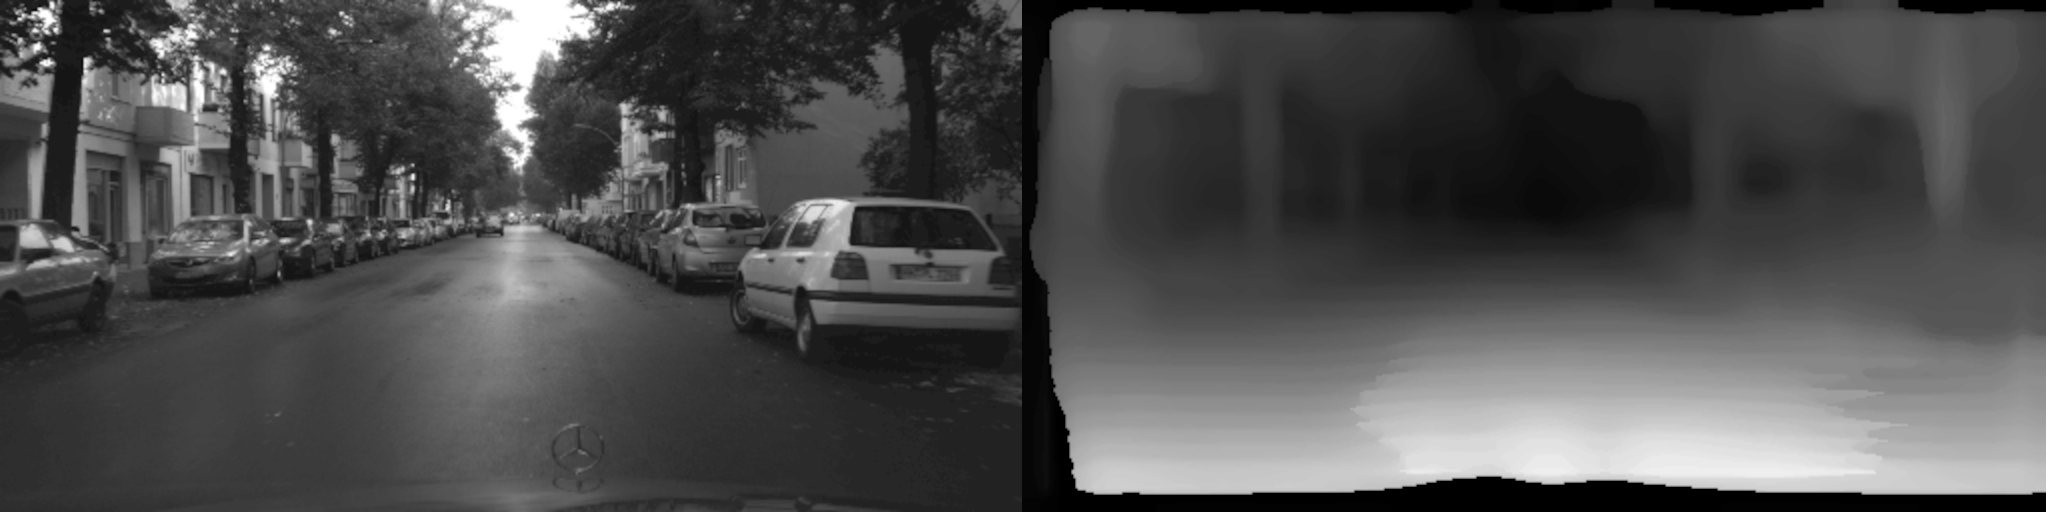
\includegraphics[width=\textwidth]{figures/new_model.png}}{uusi_malli}
\caption{Uuden mallin lopputulos}
\label{fig:uusi_malli}
\end{figure}


Vaikka malli saavuttaisikin "täydellisen" lopputuloksen, se ei silti tuota haluttuja tuloksia, koska koulutusdata ei ole täydellistä.
Tuotettu lopullinen malli onkin mielestäni tästä johtuen hyvä, vaikka sen tuottama kuva onkin "sumea". 
Tämä sumeus auttaa piilottamaan epätarkkuuksia, joka todennäköisesti tekisi mallista riittävän mahdollisissa reaalimaailman käyttökohteissa.
Kuvassa Kuva \ref{fig:uusi_malli} nähdään, että uusi malli pystyy arvioimaan syvyyden autotien sivussa olevien autojen takaa. 
Se myös pystyy joissain määrin arvioimaan autojen takana olevien puiden runkojen syvyyden. 
Lisäksi se on myöskin piilottanut autot silmämääräisesti paremmin kuin vanhassa kuvassa, jossa autojen ääriviivat olivat havaittavissa himmeästi.
